\subsection{Electron Drifting}
\label{sec:elec}
\begin{figure}[tbhp]
  \centering
  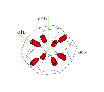
\includegraphics[width=0.4\textwidth]{valleys.eps}  
  \caption{Orientations of the crystal axes and valleys in the lab coordinate system XYZ.}
  \label{fig:valley}
\end{figure}

The dependence of the electron drift velocity $\mathbf{v}_{e}$ on the applied electric field $\mathbf{E}$ is taken to be
\begin{equation}
  \label{eq:ed}
  \mathbf{v}_{e}(\mathbf{E}) = \mathcal{A}(|\mathbf{E}|) \sum_{j} \frac{n_{j}}{n}     \frac{\gamma_{j}\mathbf{E_{0}}}     {\sqrt{\mathbf{E_{0}}\gamma_{j}\mathbf{E_{0}}}},  \mbox{ with }     j=1,2,3,4
\end{equation}
where $\mathcal{A}$ is a function of the magnitude of the electric field and temperature, the value of $\mathcal{A}$ must be negative because electrons drift to the opposite direction of the electric field; $\mathbf{E_{0}}$ is the normalized electric field vector; $n_{j}/n$ is the fraction  of the carriers (in this case, electrons) in the $j$-th valley, $\gamma_{j}$ is the effective mass tensor for the $j$-th valley. In general the tensor $j$-th is given in terms of the rotation matrices $R_{i}$, responsible for aligning the $i$-th $\langle 111 \rangle$ axis with the Y-axis of the lab system, by
\begin{equation}
  \label{eq:gammas}
  \gamma_{j} = R_{j}^{T}\gamma_{0}R_{j}, \mbox{ with } \gamma_{0}   \equiv \left(
    \begin{array}{ccc}
      m_{t}^{-1} & 0 & 0 \\
      0 & m_{l}^{-1} & 0 \\
      0 & 0 & m_{t}^{-1}
    \end{array} \right),
\end{equation}
where $m_{t} = 1.64m_{e}, m_{l} = 0.0819m_{e}$ with $m_{e}$ denoting the free electron mass, and the rotation matrix $R_{j} = R_{x^{\prime}}(\arccos(\sqrt{2/3}))R_{z}((j-1)\pi/2)$.

\begin{figure}[tbhp]
  \centering
  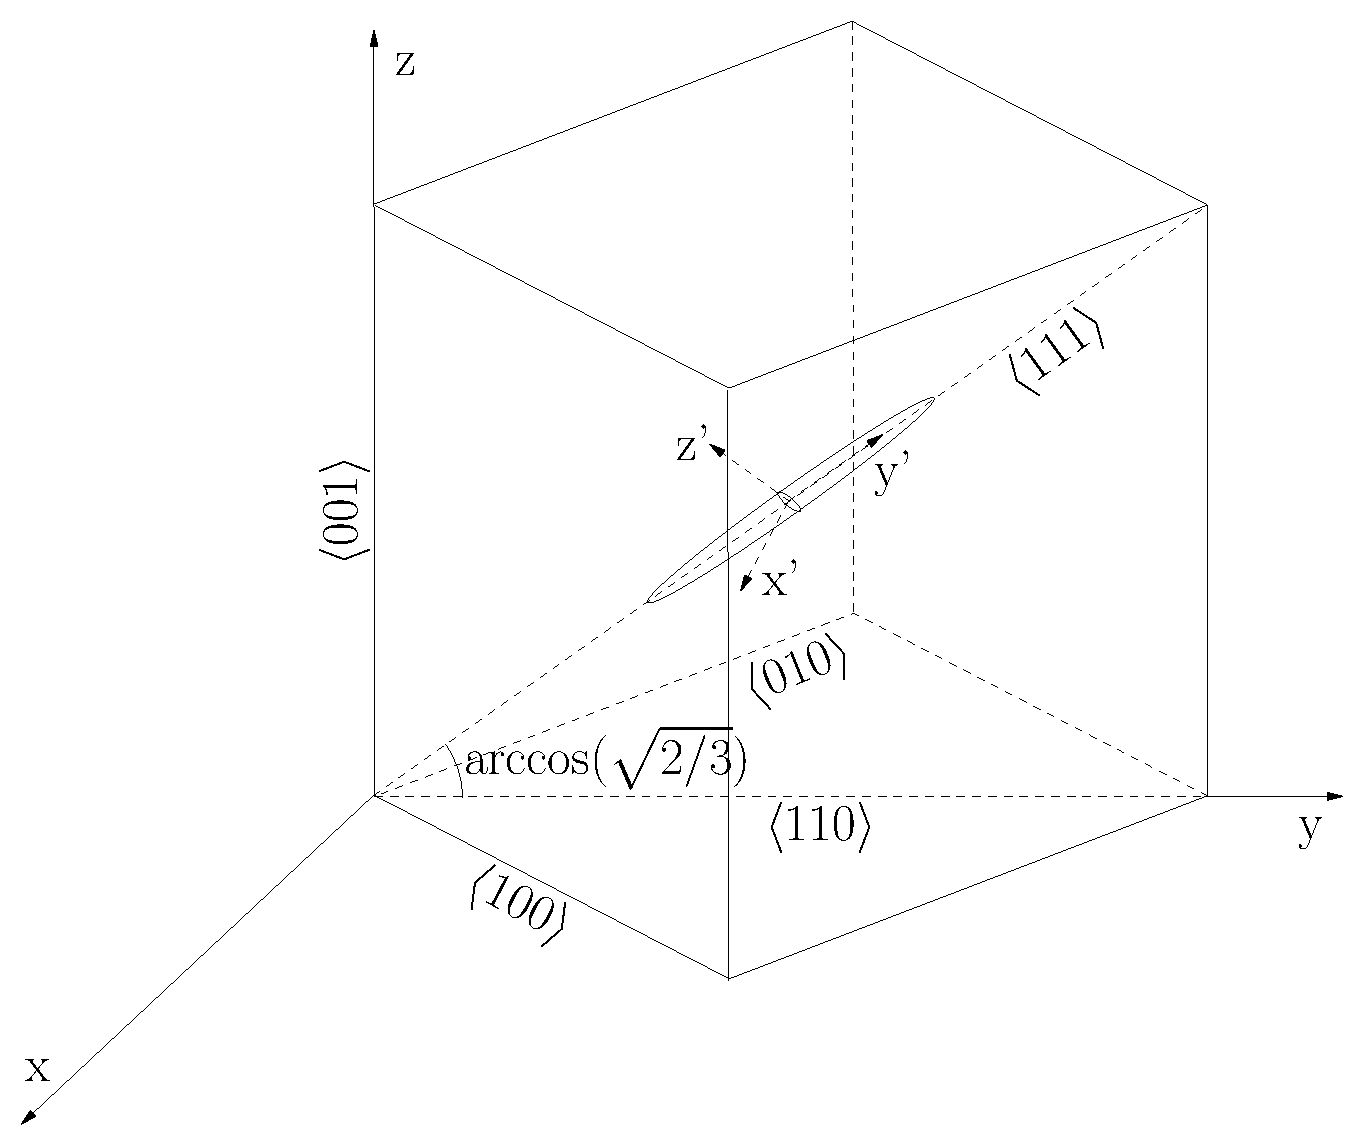
\includegraphics[width=0.6\textwidth]{axes.eps}  
  \caption{Orientations of the crystal axes and valleys in the lab coordinate system XYZ.}
  \label{fig:axes}
\end{figure}

For an experimental determination of the repopulation amplitude, the deviation from a uniform population distribution $n_{e}/n$ (1/4 for germanium) is assumed to vary with the electric field weighted by the factor $\mathcal{R}$:
\begin{equation}
  \label{eq:nion}
  \frac{n_{j}}{n} = \mathcal{R(|\mathbf{E}|)}   \left[         \frac{\sqrt{\mathbf{E_{0}}\gamma_{j}\mathbf{E_{0}}}}
    {\sum_{i}\sqrt{\mathbf{E_{0}}\gamma_{i}\mathbf{E_{0}}}} -               \frac{n_{e}}{n} \right] + \frac{n_{e}}{n},  \mbox{ with }           i=1,2,3,4
\end{equation}

If the electric field vector is equally oriented with respect to all the $\langle111\rangle$ directions, there is an uniform repopulation of the conduction bands, \textit{i.e.} $n_{j}/n = 1/4$. An electric field applied along the $\langle100\rangle$ direction, \textit{i.e.} $\mathbf{E_{0}} = (1/\sqrt{2},1/\sqrt{2},0)^{T}$, satisfies this condition. By employing the experimental drift velocity $v_{e}^{exp}(E)$ for an applied electric field $E$ in the $\langle100\rangle$ direction at a specific temperature, the absolute value  of $\mathcal{A}(|\mathbf{E}|)$ can be calculated as
\begin{equation}
  \label{eq:ae}
  \mathcal{A}(|\mathbf{E}|) = \frac{v_{e}^{exp}(E)}  {\displaystyle \sum_{j}     \frac{1}{4}     \frac{\gamma_{j}\mathbf{E_{0}}}         {\sqrt{\mathbf{E_{0}}\gamma_{j}\mathbf{E_{0}}}} },  \mbox{ with }       \mathbf{E_{0}} = \left( \begin{array}{c} 
    1/\sqrt{2}\\1/\sqrt{2}\\0 \end{array} \right).
\end{equation}

If the electric field vector is oriented along with one of the $\langle111\rangle$ directions, \textit{i.e.} $\mathbf{E_{0}} = (0,\sqrt{2}/\sqrt{3},1/\sqrt{3})^{T}$, there is an uniform repopulation of the conduction bands among the other three $\langle111\rangle$-axes, \textit{i.e.}
\begin{equation}
  \label{eq:n111}
  \frac{n_{2}}{n} = \frac{n_{3}}{n} = \frac{n_{4}}{n}.
\end{equation}
Since
\begin{equation}
  \label{eq:nsum}
  \displaystyle \sum_{j}\frac{n_{j}}{n} = 1,
\end{equation}
we have
\begin{equation}
  \label{eq:n12}
  \frac{n_{1}}{n} + 3\frac{n_{2}}{n}= 1.
\end{equation}
By employing the experimental drift velocity $v_{e}^{exp}(E)$ for an applied electric field $E$ in the $\langle111\rangle$ direction at a specific temperature, we have another relation between $n_{1}/n$ and $n_{2}/n$:
\begin{equation}
  \label{eq:n12p}
  v_{e}^{exp}(E) =  \mathcal{A}(|\mathbf{E}|) \left(  \frac{n_{1}}{n} \frac{\gamma_{1}\mathbf{E_{0}}}         {\sqrt{\mathbf{E_{0}}\gamma_{1}\mathbf{E_{0}}}} +  3\frac{n_{2}}{n} \frac{\gamma_{2}\mathbf{E_{0}}}         {\sqrt{\mathbf{E_{0}}\gamma_{2}\mathbf{E_{0}}}} \right).
\end{equation}
One can get the value of $n_{1}/n$ and $n_{2}/n$ by solving the equations \ref{eq:n12} and \ref{eq:n12p} together. Then $\mathcal{R}(|\mathbf{E}|)$ can be calculated as
\begin{equation}
  \label{eq:re}
  \mathcal{R(|\mathbf{E}|)} = \left( \frac{n_{1}}{n} - \frac{n_{e}}{n}     \right) / \left(     \frac{\sqrt{\mathbf{E_{0}}\gamma_{1}\mathbf{E_{0}}}}
    {\sum_{i}\sqrt{\mathbf{E_{0}}\gamma_{i}\mathbf{E_{0}}}} -                           \frac{n_{e}}{n} \right),  \mbox{ with }           i=1,2,3,4 \mbox{ and       } \mathbf{E_{0}} = \left( \begin{array}{c} 
      0\\ \sqrt{2}/\sqrt{3}\\1/\sqrt{3} \end{array} \right).
\end{equation}

The dependence of the experimental $\langle111\rangle$ and $\langle100\rangle$ drift velocities on the electric field can be fitted with the empirical formula: 
\begin{equation}
  \label{eq:expe}  
  v_{e}^{exp}(E) = \frac{\mu_{0}E}{(1+(E/E_{0})^{\beta})^{1/\beta}} - \mu_{n}E.
\end{equation}
The fitted parameters values are presented in Table~\ref{tab:pars}
\begin{table}[tbhp]
  \centering
  \begin{tabular}{ccccc}\hline\hline
    Direction & $\mu_{0} \left[ \frac{\mbox{cm}^{2}}{\mbox{V}\cdot\mbox{s}} \right]$ & $E_{0} \left[ \frac{\mbox{V}}{\mbox{cm}} \right]$ & $\beta$ & $\mu_{n} \left[ \frac{\mbox{cm}^{2}}{\mbox{V}\cdot\mbox{s}} \right]$ \\\hline
$\langle111\rangle$ & 40180 & 493 & 0.72 & 589 \\
$\langle100\rangle$ & 42420 & 251 & 0.87 & 62\\ \hline\hline
  \end{tabular}
  \caption{Fit parameters for the experimental drift velocities in the 
$\langle111\rangle$ and $\langle100\rangle$ directions.}
\label{tab:pars}
\end{table}

After determination of the parameters $\mathcal{A}$ and $\mathcal{R}$, the drift velocity can be calculated for any direction and any strength of the electric field.

\subsection{Hole Drifting}
\label{sec:hole}
%%% Local Variables:
%%% mode:latex
%%% TeX-master: "GSTR-08-M00x"
%%% End:
